Как известно, микролинзирование при больших размерах источника вносит несущественный вклад в блеск источника (\cite{schneider1992}). Для того, чтобы оценить размер источника, начиная с которого вкладом микролинзирования можно пренебречь, мы оценили величину стандартного отклонения микро-усилений в звездных величинах mobs как функцию размера источника. 

Для этой цели было сгенерировано 10 различных карт микрокаустик, каждая со следующими параметрами: $\sigma_*=0.4, \sigma_c = 0$, размер - $ 150 \times 150 $ радиусов Эйнштейна, разрешение - 1000x1000 пикселей. Источник моделировался кругом с постоянной поверхностной яркостью. Для различных значений радиусов источника производилась операция свёртки (\textit{convolution}) с каждой из построенных карт, в результате чего на выходе получалась новая карта с учётом неточечности источника. Далее, для каждого значения радиуса источника вычислялось стандартное отклонение  $\delta m_{o b s}$ по следующей формуле: 
\begin{equation}
\delta m_{o b s}=\sqrt{\frac{1}{N} \sum_{i=1}^{N}\left(x_{i}-\overline{x}\right)^{2}},
\end{equation}
где N - количество элементов в выборке, полученной объединением всех карт, $x_i$ - значения усилений, $\overline x$- среднее значение усиления по выборке.

Полученная зависимость приведена на Рисунке 4. Пунктирной линией показана теоретическая оценка стандартного отклонения микро-усилений для больших источников (угловой размер которых превышает 5 радиусов Эйнштейна) из работы (\cite{refsdalstabell1991}l):

\begin{equation}
\delta m_{o b s} \approx \frac{2.17 \sqrt{|\sigma|}}{\theta s}
\end{equation}
где $\sigma$ - плотность звёзд, $\theta_s$ - размер источника в единицах радиуса Эйнштейна для характерной массы звезды. Формула предполагается справедливой при $\gamma=0, \sigma < 1$. 

\begin{figure}[H]
    \centering
	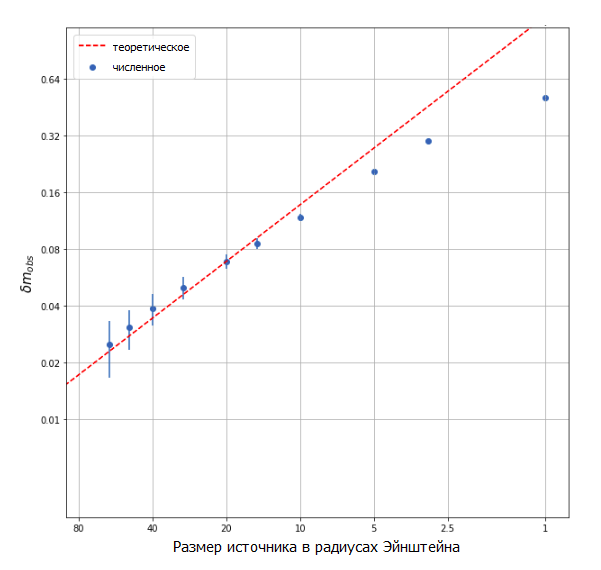
\includegraphics[scale=0.75]{pics/size_np_std.png}
	\caption{ Рис.5 Зависимость стандартного отклонения mobsот среднего значения усиления. Пунктирной линией показана теоретическая оценка $\delta m (\theta_s)$ для источников с $\theta_s > 5$(\cite{refsdalstabell1991}). Плотность звёзд: $\sigma_*=0.4$. Плотность тёмной материи и внешний сдвиг: $\sigma_с=0$.  } 
\end{figure}
Видно, что при увеличении размера источника на порядок, m уменьшается примерно так же на порядок, из чего можно сделать вывод, что для больших источников микролинзирование несущественно.